\documentclass[aspectratio=169,10pt]{beamer}
\usetheme{default}
\usecolortheme{seagull}
\setbeamertemplate{navigation symbols}{}
\setbeamertemplate{footline}[frame number]
\setbeamerfont{frametitle}{series=\bfseries,size=\large}
\setbeamercolor{frametitle}{fg=black}
\usepackage{tikz,booktabs,amsmath}
\usetikzlibrary{positioning,arrows.meta,calc}

\definecolor{cblue}{HTML}{2A78D6}
\definecolor{caqua}{HTML}{1BAF7A}
\definecolor{cyellow}{HTML}{EDA100}
\definecolor{cviolet}{HTML}{4A3AA7}
\definecolor{cred}{HTML}{E34948}
\definecolor{cgray}{HTML}{52514E}
\definecolor{cpale}{HTML}{E8E7E2}
\newcommand{\claim}[1]{\textcolor{cviolet}{\textbf{Claim:} #1}}
\newcommand{\sg}{\mathrm{sg}}

\title{Edit-JEPA:\\ Latent World Models over Text Buffers}
\subtitle{Latent planning over mutable text buffers}
\author{TextJEPA project}
\date{July 13, 2026 \quad (repo: \texttt{TextJEPA/}, runs: \texttt{runs/edit\_*})}

\begin{document}
\frame{\titlepage}

\begin{frame}{Idea: the world is a mutable draft}
\begin{itemize}\itemsep2pt
  \item State = a \textbf{text buffer}: a draft solution to an iGSM-style
        problem (same generator as the discourse track; see companion deck
        for the problem sampler).
  \item Action = a \textbf{span edit} with an intent phrase that never leaks
        outcomes: \texttt{delete step 3 .}\ /
        \texttt{insert green lamps at the start .}\ /
        \texttt{replace step 2 : recompute dark cups .}
  \item Corruptions have \textbf{propagated consequences}: corrupting one
        step's value rewrites every downstream step \emph{consistently}
        (change an assumption $\to$ later derivations change). One root cause
        $\Rightarrow$ several defects.
  \item Defect definition (symbolic, order-insensitive): a buffer step whose
        sentence $\neq$ the true step sentence, a missing necessary step, or
        an extra distractor step. \textbf{Solved} $=$ zero defects.
  \item Generation = \textbf{edit until perfect}: latent search over
        candidate edits, execute best, re-encode, repeat.
\end{itemize}
\end{frame}

\begin{frame}[fragile]{Corruption model (exact) and a verbatim sample}
\small
From the perfect draft (necessary steps, topological order), sample
independently: $k_{\text{wrong}}\sim\mathcal U\{0..2\}$ internal steps get a
wrong stated value (propagated to descendants via the corrupted value map);
$k_{\text{miss}}\sim\mathcal U\{0,1\}$ necessary steps removed;
$k_{\text{extra}}\sim\mathcal U\{0,1\}$ distractor steps inserted;
re-corrupt if defect count $=0$.
Repair trajectories: uniformly random fixing edit per step; with $p{=}0.1$
(0.25 in \texttt{valgrad}/\texttt{anchor}; max 1--2) a \textbf{vandal} edit
(harmful distractor insert) $\Rightarrow$ the value head sees edits that
\emph{increase} distance.
\medskip
\footnotesize
\textbf{Corrupted draft} (3 defects; step 3's wrong value propagates into step 4):
\begin{quote}\ttfamily
{}[1] so the number of large shells is 11 .\\
{}[2] so the number of silver cards is 17 .\\
{}[3] so the number of green books is 11 minus 17 = 5 . \textcolor{cred}{$\leftarrow$ wrong (true: 17)}\\
{}[4] so the number of golden bells is 5 times 17 = 9 . \textcolor{cred}{$\leftarrow$ consistent-but-wrong}\\
\textcolor{cgray}{missing: the step for green lamps}
\end{quote}
\textbf{Fixing intents}: \texttt{replace step 3 : recompute green books .}\quad
\texttt{insert green lamps at the start .}
\end{frame}

\begin{frame}{Architecture: slot-based buffer encoder + shared JEPA core}
\begin{columns}
\column{0.55\textwidth}\footnotesize
\begin{itemize}\itemsep2pt
  \item Chunk encoder $E_c$ (identical to discourse track, 256-d).
  \item \textbf{SlotBufferEncoder}: 4 learned slot queries cross-attend
        over prompt and position-encoded buffer sentences; four flattened
        slots form the 256-d state.
  \item The action encoder, latent predictor $F$, displacement decoder,
        hierarchical objective, and value head are shared with the discourse
        architecture.
  \item Value target = \textbf{defects remaining} (distance to perfect).
  \item \textbf{Fixed outcome target}: predict a frozen random-feature
        embedding of the post-edit buffer from $(s_t,a_t)$.
  \item \textbf{Sentence-attentive transition}: action-conditioned queries
        attend to individual buffer sentences before next-state prediction,
        avoiding a purely pooled transition bottleneck.
\end{itemize}
\column{0.43\textwidth}
\centering
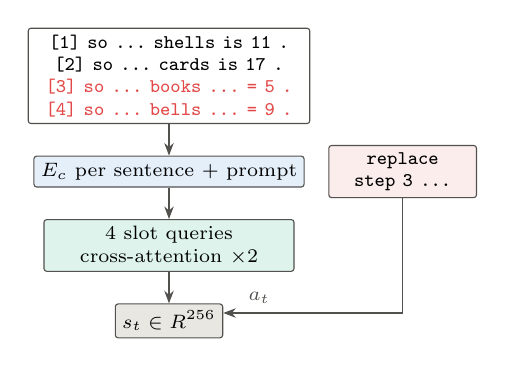
\begin{tikzpicture}[font=\scriptsize,
  box/.style={draw=cgray, rounded corners=1pt, inner sep=2.5pt, align=center},
  arr/.style={-{Stealth[length=1.6mm]}, cgray}]
\node[box, fill=white, text width=34mm] (buf) at (0,0)
  {\ttfamily [1] so ...\ shells is 11 .\\{}
   [2] so ...\ cards is 17 .\\{}
   \textcolor{cred}{[3] so ...\ books ...\ = 5 .}\\{}
   \textcolor{cred}{[4] so ...\ bells ...\ = 9 .}};
\node[box, fill=cblue!12, below=4mm of buf] (ec) {$E_c$ per sentence + prompt};
\node[box, fill=caqua!15, below=4mm of ec, text width=30mm]
  (slots) {4 slot queries\\ cross-attention $\times2$};
\node[box, fill=cpale, below=4mm of slots] (s) {$s_t \in \mathbb R^{256}$};
\node[box, fill=cred!10, right=3mm of ec, text width=17mm]
  (edit) {\ttfamily replace step 3 ...};
\draw[arr] (buf) -- (ec); \draw[arr] (ec) -- (slots);
\draw[arr] (slots) -- (s);
\draw[arr] (edit) |- ($(s.east)+(0,0.1)$)
  node[pos=0.9, above, font=\scriptsize]{$a_t$};
\end{tikzpicture}
\end{columns}
\end{frame}

\begin{frame}{Objectives, training, planning}
\small
\textbf{Losses}: identical composite to the discourse deck (weights 1.0
pred / 1.0 rollout / 0.5 hierarchy / 1.0 VICReg / 2.0 Delta-JEPA / 1.0
value; \texttt{anchor} adds $\mathcal L_{\text{chunk}}$ w=2.0 on frozen
buffer embeddings). Labels: op $\in$ \{delete, insert, replace\}; ``was the
edit a fix or vandalism'' plays the goal-relevance role.
\smallskip

\textbf{Training}: batch 64 (each item encodes all $T{+}1$ buffer
snapshots), 20 epochs over a deterministic 60k-trajectory corpus, otherwise identical
protocol (AdamW $3{\times}10^{-4}$, EMA $0.99{\to}0.999$, RTX 6000,
$\sim$70--90 min).
\smallskip

\textbf{Planning}: candidates from the edit interface = \{delete
$p$, replace $p$\} for every position $+$ insert for every missing necessary
step $+$ 2 harmful distractor inserts (planner must \emph{reject} them);
score $V(F(s,a_i), s_{\text{init}})$; apply argmin in the environment;
re-encode; budget $=$ initial defects $+$ slack.
Success $=$ \textbf{perfect draft within the optimal number of edits}.
\end{frame}

\begin{frame}{Result --- the geometry was never the problem}
\begin{columns}
\column{0.5\textwidth}
\centering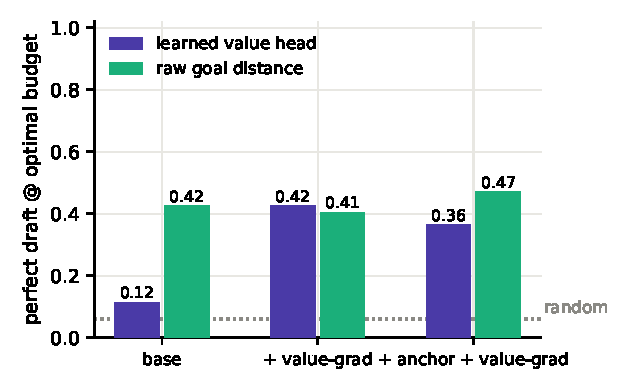
\includegraphics[width=\linewidth]{figs/edit_planning.pdf}
\column{0.48\textwidth}\small
\claim{The buffer encoder's \emph{raw} goal-distance geometry beats every
learned edit value head --- the published weakness was a value-head
failure.}
\begin{itemize}\itemsep2pt
  \item Value heads: latent-prediction baseline 0.115 (random 0.06),
        end-to-end value shaping 0.425, fixed outcome target 0.365 --- all
        \textbf{slack-insensitive} (ties on no-op edits waste budget).
  \item Raw goal distance $\|\mathrm{LN}(\hat s)-\mathrm{LN}(s_{\text{goal}})\|_1$
        ($s_{\text{goal}}$ = encoded perfect buffer): latent-prediction
        baseline \textbf{0.425}, fixed outcome target \textbf{0.47} --- $4\times$ the
        base value head, no value supervision used at plan time.
  \item Geometry regularizers (straighten/monotonicity, cf.\ discourse
        deck) change nothing here: 0.445--0.485 ---
        corr($d^{\text{goal}}$, defects) was already $\approx$0.75.
\end{itemize}
\end{columns}
\end{frame}

\begin{frame}{Result 2 --- preference learning and transition architecture}
\claim{Counterfactual preference learning makes planning slack-sensitive;
sentence-level attention then improves transition matching and planning.}
\centering\scriptsize
\begin{tabular}{lccccc}
\toprule
 & \multicolumn{2}{c}{value energy} & goal dist. & value $\tau$ & matching\\
run & @opt & @slack2 & @opt & (audit) & (chance .10)\\
\midrule
fixed outcome target & 0.365 & 0.375 & 0.47 & 0.39 & 0.47\\
counterfactual preference ($K=4$) & 0.46 & 0.505 & \textbf{0.60}
 & 0.59 & 0.43\\
\textbf{attention transition model} & \textbf{0.51} & \textbf{0.55} & 0.535
 & \textbf{0.61} & \textbf{0.50}\\
geometry-distilled value & 0.42 & 0.42 & 0.55 & 0.42 & 0.45\\
without harmful-edit negatives & 0.22 & 0.225 & 0.445 & $-$0.07 & 0.39\\
five-objective model (no defect counts) & 0.455 & 0.485 & 0.545 & --- & ---\\
\bottomrule
\end{tabular}

\medskip\small
\textbf{Readings.} Preference learning gives the first slack-sensitive edit
planner. Action-conditioned attention over individual sentences raises the
learned-value planner from 0.46/0.505 to 0.51/0.55 and matching from 0.43 to
0.50. Geometry-distilled $V$ matches scalar defect-count supervision (0.42 vs
0.425), while removing harmful-edit negatives makes the energy anti-correlated
($\tau=-0.07$). Matching remains below the discourse track's 1.00, so transition
fidelity still limits the edit model.
\end{frame}

\begin{frame}{Probe summary (edit track)}
\centering\small
\begin{tabular}{lccc}
\toprule
probe (linear, validation split) & baseline & value shaping & random encoder\\
\midrule
edit op from $\Delta s$ & 1.00 & 1.00 & 1.00$^*$\\
fix-vs-vandal from $\Delta s$ & 0.96 & 0.98 & 0.92\\
defects remaining from $s_t$ & 0.46 & --- & 0.38\\
buffer length from $s_t$ & 0.91 & --- & 0.73\\
claimed answer from $s_t$ & 0.23 & --- & 0.28\\
true answer from terminal state & 0.05 & --- & 0.13\\
\bottomrule
\end{tabular}

\medskip\small
$^*$intent phrases are trivially separable by op --- the informative row is
fix-vs-vandal. The two bottom rows show the \textbf{collusion signature}
(trained $<$ random control): outcome content is being smoothed away, as in
the discourse track before adding a fixed outcome target. The corresponding
edit model (weight 2.0) trains $\mathcal L_{\text{chunk}}$ to 0.005 and lifts
value-head planning to 0.365, but the linear \emph{defect-count} probe stays
flat --- the goal signal lives in the \emph{metric} (see previous slide),
not in a linearly decodable counter.
\end{frame}

\begin{frame}{Diagnosis \& next steps}
\begin{itemize}\itemsep2pt
  \item \textbf{Why the base value head fails}: repairs are
        near-deterministic given the defect set, so state prediction is easy
        without a linear defect counter; but the \emph{metric} structure
        (distance to the perfect buffer) is there from the start --- use the
        goal-distance energy, or distill it into $V$.
  \item \textbf{Deployable goal states}: the oracle goal uses the true
        buffer; a deployable version needs a goal \emph{description} encoder
        (``all steps correct'') or a self-predicted fixed point
        $F(s,a_{\text{stop}}) \approx s$.
  \item \textbf{Energy ties}: counterfactual preferences make success
        slack-sensitive. Sentence-level attention raises matching
        0.43$\to$0.50 and planning 0.46/0.505$\to$0.51/0.55, but the remaining
        gap to discourse matching indicates that transition fidelity still binds.
  \item \textbf{Harder corruption}: multiple root causes, order violations,
        subtle wrong-parent corruptions (currently only wrong values /
        missing / extra).
  \item \textbf{Long-term}: draft-level macro edits (rewrite region), and the
        hierarchical planner shared with the discourse track.
\end{itemize}
\end{frame}

\end{document}
